\clearpage
%3.5
\subsection{スクリプトの\ruby{保存}{ほ|ぞん}}

最後に自分で書き換えたスクリプトを保存する方法を忘れずに覚えておきましょう。
スクリプトをファイルとして保存しておけば、いつでも開いて続きから始めることができます。ファイル→「名前を付けて保存…」から、「mygpio.hsp」など自分の好きな名前で保存しておいてください。

\begin{figure}[H]
    \begin{center}
        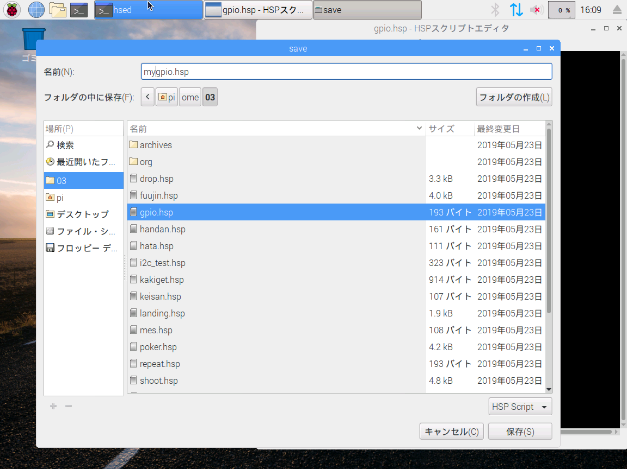
\includegraphics[keepaspectratio,width=6.976cm,height=4.944cm]{text02-img/text02-img028.png}
        \caption{スクリプト保存のダイアログ}
    \end{center}
\end{figure}

\subsection{例題に挑戦しよう}

ここまで終わってしまった人は、以下の例題にも挑戦してみよう。

\begin{itemize}
    \item 命令のヘルプと検索のしかたを覚える
    \item 文字に色をつけてみる(color命令)
    \item 文字の位置やサイズを変えてみる(pos,font命令)
    \item 四角形を描く命令を使ってみる(boxf命令)
\end{itemize}

例題の考え方がわからない時は、近くのTAか先生に聞いてください。
わからない所は、そのままにせず、必ず答えを見つけてから先に進みましょう。

\clearpage
\subsection{例題5 命令のヘルプと\ruby{検索}{けん|さく}のしかたを覚える}

\subsubsection*{考え方}

HSPで使うことのできる命令を調べたり、説明を読むための方法を覚えておきましょう。
HSPで書ける命令は、色々な種類があります。HSPスクリプトエディタで調べたい命令にカーソルを合わせて[F1]キーを押すことでヘルプが表示されます。

左上の入力枠に命令を入れて検索をすることができます。
試しに、「mes」「wait」などの命令を調べてみましょう。

\subsubsection*{例題5 答え}

mes命令のヘルプが正しく表示されたかどうか確認してみましょう。
このページでは、HSPの命令やサンプル、\ruby{関連}{かん|れん}する命令などを検索することができます。

\begin{figure}[H]
    \begin{center}
        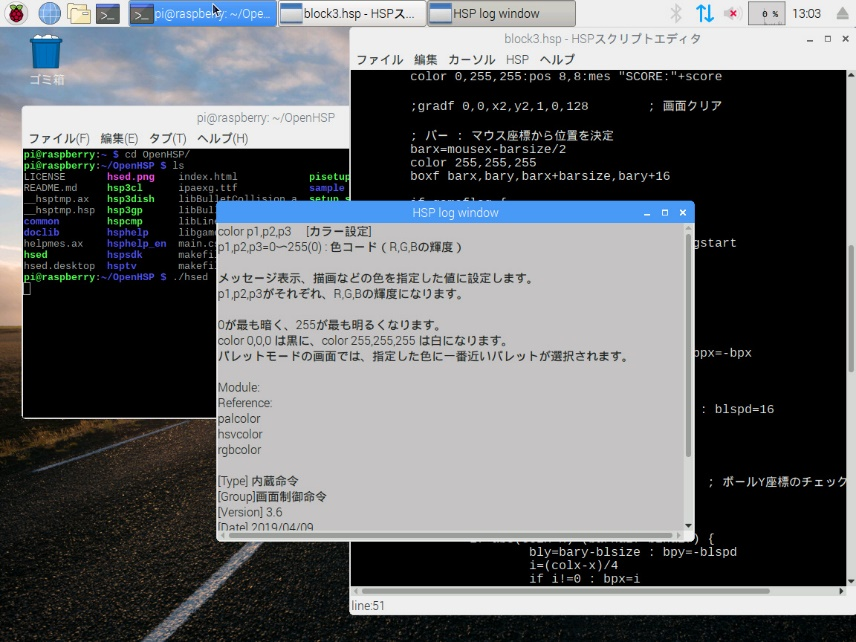
\includegraphics[keepaspectratio,width=9.895cm,height=7.421cm]{text02-img/text02-img029.jpg}
        \caption{ヘルプの画面}
    \end{center}
\end{figure}